\chapter{Descriptive overview of Edit Filters on the English Wikipedia}
\label{chap:overview-en-wiki}

The purpose of this chapter (syn?) is to explore the edit filters on the Englisch Wikipedia.
We want to gather a understanding of what types of tasks these filters take over,
and, as far as feasible, trace how these tasks have evolved over time.

%TODO describe what each section is about
The data upon which the analysis is based is described in section~\ref{sec:overview-data}
and the methods we use–in chapter 3.
Section~\ref{sec:patterns} explores (syn) some patterns in the edit filters' usage and..
And we look into the manual classification of EN Wikipedia's edit filters I've undertaken in an attempt to understand what is it that they actually filter in section~\ref{sec:manual-classification}.


\section{Data}
\label{sec:overview-data}

The main part of the present analysis rests upon/is based upon/is grounded in/foundations lie the \emph{abuse\_filter} table from \emph{enwiki\_p}(the database which stores data for the EN Wikipedia), or more specifically a snapshot thereof which was downloaded on January 6th, 2019 via quarry, a web-based service offered by Wikimedia for running SQL queries against their public databases~\footnote{\url{https://quarry.wmflabs.org/}}.
The complete dataset can be found in the repository for the present paper~\cite{github}. % TODO add a more specific link

This table, along with \emph{abuse\_filter\_actions}, \emph{abuse\_filter\_log}, and \emph{abuse\_filter\_history}, are created and used by the AbuseFilter MediaWiki extension~\cite{gerrit-abusefilter-tables}, as discussed in section~\ref{sec:mediawiki-ext}.
Selected queries have been run via quarry against the \emph{abuse\_filter\_log} table as well.
Unfortunately, the \emph{abuse\_filter\_history} table which will be necessary for a complete historical analysis of the edit filters is currently not exposed to the public due to security/privacy concerns~\cite{phabricator}.
Therefore, the present work only touches upon historical trends in a qualitative fashion. %TODO how are these determined: API to abuse_filter_history; general stats from abuse_filter
or qualitatively shows patterns.
A comprehensive historical analysis is therefore (syn!) one of the possibilities/directions for future studies (syn).

%TODO maybe move to appendix; mention tables have been discussed in~\ref{sec:mediawiki-ext} and only quote here the one for abuse\_filter since we are using the data
A concise description of the tables has been offered in section~\ref{sec:mediawiki-ext} which discusses the AbuseFilter MediaWiki extension in more detail.
Here, only the schema of the \emph{abuse\_filter} table has been included (figure~\ref{fig:db-schemas-af}), since that is the data the present analysis is based upon.
For further reference, the schemas of all four tables can be viewed in figures~\ref{fig:app-db-schemas-af},~\ref{fig:app-db-schemas-afl},~\ref{fig:app-db-schemas-afh} and~\ref{fig:app-db-schemas-afa} in the appendix.

\begin{figure*}
\begin{verbatim}
abuse_filter
+--------------------+----------------+------+-----+---------+----------------+
| Field              | Type           | Null | Key | Default | Extra          |
+--------------------+----------------+------+-----+---------+----------------+
| af_id              | bigint(20)     | NO   | PRI | NULL    | auto_increment |
| af_pattern         | blob           | NO   |     | NULL    |                |
| af_user            | bigint(20)     | NO   | MUL | NULL    |                |
| af_user_text       | varbinary(255) | NO   |     | NULL    |                |
| af_timestamp       | binary(14)     | NO   |     | NULL    |                |
| af_enabled         | tinyint(1)     | NO   |     | 1       |                |
| af_comments        | blob           | YES  |     | NULL    |                |
| af_public_comments | tinyblob       | YES  |     | NULL    |                |
| af_hidden          | tinyint(1)     | NO   |     | 0       |                |
| af_hit_count       | bigint(20)     | NO   |     | 0       |                |
| af_throttled       | tinyint(1)     | NO   |     | 0       |                |
| af_deleted         | tinyint(1)     | NO   |     | 0       |                |
| af_actions         | varbinary(255) | NO   |     |         |                |
| af_global          | tinyint(1)     | NO   |     | 0       |                |
| af_group           | varbinary(64)  | NO   | MUL | default |                |
+--------------------+----------------+------+-----+---------+----------------+
\end{verbatim}
  \caption{abuse\_filter schema}~\label{fig:db-schemas-af}
\end{figure*}

\section{Descriptive statistics/Patterns}
\label{sec:patterns}

In this section, we explore some general patterns of the edit filters on Engish Wikipedia, or respectively the data from the \emph{abuse\_filter} table.
The scripts that generate the statistics discussed here, can be found in the jupyter notebook in the project's repository. %TODO add link after repository has been cleaned up

As of January 6th, 2019 there are 954 filters in this table.
It should be noted, that if a filter gets deleted, merely a flag is set to indicate so, but no entries are removed from the database.
So, the above mentioned 954 filters are all filters ever made up to this date.
This doesn't mean that it never changed what the filters are doing, since, as pointed out in chapter~\ref{}, edit filter managers can freely modify filter patterns, so at some point the filter could be doing one thing and in the next moment, it is filtering a completely different phenomenon.
This doesn't happen very often though.

Tables ... show how many new filters have been introduced over the years.
And how many filters have been active (``enabled'') over the years. %TODO do I have data for this

Thanks to quarry, we have all the filters that were triggered from the filter log per year, from 2009 (when filters were first introduced/the MediaWiki extension was enabled) till end of 2018 with their corresponding number of times being triggered:
Table~\ref{tab:active-filters-count} summarises the numbers of distinct filters that got triggered over the years.
So, the number of distinct filters that have been triggered over the years varies between 154 in year 2014 and 254 in 2018.
This is not a terrible wide range and the probable explanation to this is the so-called condition limit.
%TODO: number of filters cannot grow endlessly, every edit is checked against all of them and this consumes computing power! (and apparently haven't been chucked with Moore's law). is this the reason why number of filters has been more or less constanst over the years?
\begin{comment}
\url{https://en.wikipedia.org/wiki/Wikipedia:Edit_filter/Requested}
"Each filter takes time to run, making editing (and to some extent other things) slightly slower. The time is only a few milliseconds per filter, but with enough filters that adds up. When the system is near its limit, adding a new filter may require removing another filter in order to keep the system within its limits."
\end{comment}

\begin{table}
  \centering
  \begin{tabular}{l r }
    % \toprule
    Year & Num of distinct filters \\
    \hline
    2009 & 220 \\
    2010 & 163 \\
    2011 & 161 \\
    2012 & 170 \\
    2013 & 178 \\
    2014 & 154 \\
    2015 & 200 \\
    2016 & 204 \\
    2017 & 231 \\
    2018 & 254 \\
    % \bottomrule
  \end{tabular}
  \caption{Count of distinct filters that got triggered each year}~\label{tab:active-filters-count}
\end{table}

We can follow/track/backtrack the number of filter hits over the years (syn) on figure~\ref{fig:filter-hits}.
There is a dip in the number of hits in late 2014 and quite a surge in the beginnings of 2016.
Here is the explanation to that:
%TODO discuss peak! (and overall pattern)
%TODO strectch plot so months are readable
\begin{figure}
\centering
  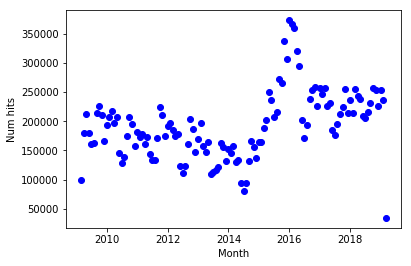
\includegraphics[width=0.9\columnwidth]{pics/number-filter-hits.png}
  \caption{EN Wikipedia edit filters: Number of hits per month}~\label{fig:filter-hits}
\end{figure}

\begin{comment}
    \item has the willingness of the community to use filters increased over time?: looking at aggregated values of number of triggered filters per year, the answer is rather it's quite constant; TODO: plot it at a finer granularity
        when aggregating filter triggers per month, one notices that there's an overall slight upward tendency.
\end{comment}

The ten most active filters of all times (with number of hits and public description) are displayed in table~\ref{tab:most-active-actions}.
For a more detailed reference, the ten most active filters of each year are listed in the appendix. %TODO are there some historical trends we can read out of it?
and, of course, the whole table can be consulted in the repository~\cite{github}.
\begin{table*}
  \centering
    \begin{tabular}{r r p{10cm} p{2cm} }
    % \toprule
        Filter ID & Hitcount & Publicly available description & Actions \\
    \hline
       61 & 1,611,956 & new user removing references & tag \\
      135 & 1,371,361 & repeating characters & tag, warn \\
      527 & 1,241,576 & T34234: log/throttle possible sleeper account creations (hidden filter) & throttle \\
      384 & 1,159,239 & addition of bad words or other vandalism & disallow \\
      172 & 935,925 & section blanking & tag \\
       30 & 840,871 & large deletion from article by new editors & tag, warn \\
      633 & 808,716 & possible canned edit summary & tag \\
      636 & 726,764 & unexplained removal of sourced content & warn \\
        3 & 700,522 & new user blanking articles & tag, warn \\
      650 & 695,601 &creation of a new article without any categories & (log only) \\
  \end{tabular}
  \caption{What do most active filters do?}~\label{tab:most-active-actions}
\end{table*}

%TODO compare with table and with most active filters per year: is it old or new filters that get triggered most often? (I'd say it's a mixture of both and we can now actually answer this question with the history API, it shows us when a filter was first created)

\begin{comment}
    \item how many currently trigger which action (disallow, warn, throttle, tag, ..)?
    \item how often were filters with different actions triggered? (afl\_actions) (over time) --> abuse\_filter\_log
    \item explore timestamp (I think it means "last modified"): have a lot of filters been modified recently?
    \item categorise filters according to which name spaces they apply to; pay special attention to edits in user/talks name spaces (may be indication of filtering harassment)
\end{comment}


\begin{comment}
\textbf{Questions on abuse\_filter\_log table}
\begin{itemize}
    \item how often were filters with different actions triggered? (afl\_actions)
    \item what types of users trigger the filters (IPs? registered?) : IPs: 16,489,266, logged in users: 6,984,897 (Stand 15.03.2019);
    \item on what articles filters get triggered most frequently (afl\_title)
    \item what types of user actions trigger filters most frequently? (afl\_action) (edit, delete, createaccount, move, upload, autocreateaccount, stashupload)
    \item in which namespaces get filters triggered most frequently?
\end{itemize}

\textbf{Questions on abuse\_filter\_action table}
\begin{itemize}
    \item how many filters trigger any particular action (at the moment)?
    \item how many different parameters are there (i.e. tags when tagging, or templates to show upon a warning)?
\end{itemize}
\end{comment}

\textbf{what do the most active filters do?}


Investigating pick in filter hits beginnings of 2016

Looking at january 2016:

till now it comes to attention that a lot of accounts named something resembling <FirstnameLastname4RandomLetters> were trying to create an account  (while logged in?) (or maybe it was just that the creation of these particular accounts itself was denied); this triggers filter 527 ("T34234: log/throttle possible sleeper account creations
")
There are in the meantime over 5 pages of them, it is definitely happening automatically

TODO: download data; write script to identify actions that triggered the filters (accountcreations? edits?) and what pages were edited

\begin{comment}
It is not, as some seem to believe, intended to block profanity in articles (that would be extraordinarily dim), nor even to revert page-blankings. That's what we have ClueBot and TawkerBot for, and they do a damn good job of it. This is a different tool, for different situations, which require different responses. I conceive that filters in this extension would be triggered fewer times than once every few hours. — Werdna • talk 13:23, 9 July 2008 (UTC) "
// longer clarification what is to be targeted. interestingly enough, I think the bulk of the things that are triggered today are precisely the ones Werdna points out as "we are not targeting them".
%TODO Compare with most active filters
\end{comment}

A lot of filters are disabled/deleted bc:
* they hit too many false positives: 14 (disabled in couple of hours)
* they were implemented to target specific incidents and these vandalism attempts stopped :663
* they were tested and merged into other filters
* there were too few hits and the conditions were too expensive

Multiple filters have the comment "let's see whether this hits something", which brings us to the conclusion that edit filter editors have the right and do implement filters they consider necessary


%\subsection{Types of edit filters}
%We can sort filters into categories along various criteria.
%For now we don't have a different criteria...

\section{Public and Hidden Filters}

The first noticeable typology is along the line public/private filters.

It is calling attention that nearly 2/3 of all edit filters are not viewable by the general public.
%TODO: remark that it was to investigate this historically; or is there still an easy way to do this?

The guidelines call for hiding filters ``only where necessary, such as in long-term abuse cases where the targeted user(s) could review a public filter and use that knowledge to circumvent it.''~\cite{Wikipedia:EditFilter}.
Further, they suggest caution in filter naming and giving just simple description of the overall disruptive behaviour rather than naming specific user that is causing the disruptions.
(The later is not always complied with, there are indeed filters named after the accounts causing a disruption.)

Only edit filter editors (who have the \emph{abusefilter-modify} permission) and editors with the \emph{abusefilter-view-private} permission can view hidden filters.
The later is given to edit filter helpers - editors interested in helping with edit filters who still do not meet certain criteria in order to be granted the full \emph{abusefilter-modify} permission, editors working with edit filters on other wikis interested in learning from the filter system on English Wikipedia, and Sockpuppet investigation clerks~\cite{Wikipedia:EditFilterHelper}.
As of March 17, 2019, there are 16 edit filter helpers on EN Wikipedia~\footnote{\url{https://en.wikipedia.org/wiki/Special:ListUsers/abusefilter-helper}}.
Also, all administrators are able to view hidden filters.

There is also a designated mailing list for discussing these: wikipedia-en-editfilters@lists.wikimedia.org.
It is specifically indicated that this is the communication channel to be used when dealing with harassment (by means of edit filters)~\cite{Wikipedia:EditFilter}.
It is signaled, that the mailing list is meant for sensitive cases only and all general discussions should be held on-wiki~\cite{Wikipedia:EditFilter}.

\begin{comment}
https://en.wikipedia.org/wiki/Wikipedia_talk:Edit_filter/Archive_1
// so, according to Werdna, main targetted group are especially determined vandals in which case it makes sense to hide filters' heuristics from them. Which would also explain why 2/3 of the filters are hidden

\url{https://en.wikipedia.org/wiki/Wikipedia:Edit_filter}
"Non-admins in good standing who wish to review a proposed but hidden filter may message the mailing list for details."
// what is "good standing"?
// what are the arguments for hiding a filter? --> particularly obnoctious vandals can see how their edits are being filtered and circumvent them; security through obscurity -- compare also comments on the TalkPage; this is not crypto.
// are users still informed if their edit triggers a hidden filter? - most certainly; the warnings logic has nothing to do with whether the filter is hidden or not

"For all filters, including those hidden from public view, a brief description of what the rule targets is displayed in the log, the list of active filters, and in any error messages generated by the filter. " //yeah, well, that's the public comment, aka name of the filter

"Be careful not to test sensitive parts of private filters in a public test filter (such as Filter 1): use a private test filter (for example Filter 2) if testing is required."

\end{comment}

\section{Types of edit filters: Manual Classification}
\label{sec:manual-classification}

Apart from filter typologies that can be derived directly from the DB schema (available fields/existing features), we propose a manual classification of the types of edits edit filters found on the EN Wikipedia target (there are edit filters with different purposes).

Based on the GT methodology, I scrutinised all filters, with their patterns, comments and actions. %TODO define more precisely what exactly are we studying
We found 3 big clusters of filters that we labeled ``vandalism'', ``good faith'' and ``maintenance''.
It was not always a straightforward decision to determine what type of edits a certain filter is targeting.
This was of course, particularly challenging for private filters where only the public comment (name) of the filter was there to guide us.
On the other hand, guidelines state up-front that filters should be hidden only in cases of particularly persistent vandalism, in so far it is probably safe to establish that all hidden filters target some type of vandalism.
However, the classification was difficult for public filters as well, since oftentimes what makes the difference between a good-faith and a vandalism edit is not the content of the edit but the intention of the editor.
While there are cases of juvenile vandalism (putting random swear words in articles) or characters repetiton vandalism which are pretty obvious, that is not the case for sections or articles blanking for example. %TODO explain why
In such ambiguous cases, we can be guided by the action the filter triggers (if it is ``disallow'' the filter is most probably targeting vandalism).
At the end, we labeled most ambiguous cases with both ``vandalism'' and ``good faith''.

In the subsections that follow we discuss the salient properties of each manually labeled category.

\begin{comment}
    \item how often were (which) filters triggered: see \url{filter-lists/20190106115600_filters-sorted-by-hits.csv} and~\ref{tab:most-active-actions}; see also jupyter notebook for aggregated hitcounts over tagged categories
    \item percentage filters of different types over the years: according to actions (I need a complete abuse\_filter\_log table for this!); according to self-assigned tags %TODO plot!
\end{comment}

Following filter categories have been identified (sometimes, a filter was labeled with more than one tag):
%TODO make a diagramm with these
- Vandalism
  - hoaxing
  - silly vandalism (e.g. repeating characters, inserting swear words)
  - spam
  - sockpuppetry
  - long term abuse // there seems to be separate documentation for this, see notes;
  - harassment/personal attacks
    - doxxing
    - impersonation
  - trolling
  - copyright violation

  Labeled along the vandalism typology (check above)
  - link vandalism
  - abuse of tags
  - username vandalism
  - image vandalism
  - avoidant vandalism
  - talk page vandalism
  - page move vandalism
  - template vandalism
  - vandalbots

  Kind of similar:
  - seo
  - stockbroker vandalism
  - biased pov
  - self promotion
  - conflict of interest

Inbetween
- edit warring
- political controversy
- politically/religiously motivated hate

- Good faith
  - bad style ("unencyclopedic edits" e.g. citing a blog or mentioning a hypothetical future album release)
  - lazyness


- Maintenance
  - bugs
  - wiki policy (compliance therewith)
  - test filters

%TODO: develop and include memos
\subsection{Vandalism}
\begin{comment}
# Filters targetting vandalism

The vast majority of edit filters on EN Wikipedia could be said to target (different forms of) vandalism.
Examples herefor are filters for *juvenile* types of vandalism (inserting swear or obscene words or nonsence sequences of characters into articles), for *hoaxing* or for *link spam*.
In principle, one can open quite a few subcategories here (also check https://en.wikipedia.org/wiki/Wikipedia:Vandalism for a "in-house" classification of vandalism types on Wikipedia).
Some vandalism types seem to be more severe than others (*sock puppetry* or persistant *long term* vandals).
For these, often times, the implemented filters are **private**.
This means, only edit filter editors can view the exact filter pattern or the comments of these.
Although this clashes with the overall *transparency* of the project (is there a guideline subscribing to this value? couldn't find a specific mention), the reasoning here is that otherwise, persistent vandals will be able to check for the pattern of the filter targetting their edits and just find a new way around it~\cite{Wikipedia:EditFilter}. %TODO compare with https://en.wikipedia.org/w/index.php?title=Wikipedia:About&oldid=891256910 about transparency as a value
There are also private filters targetting personal attack or abuse cases.
Here, filters are private in order to protect the affected person(s)~\cite{Wikipedia:EditFilter}.

The current state is also an "improvement" compared to the initially proposed visibility level of edit filters.
In the initial version of the EditFilters Page (https://en.wikipedia.org/w/index.php?title=Wikipedia:Edit_filter&oldid=221158142) Andrew Garrett (User:Werdna), the author of the AbuseFilter MediaWiki extension, was suggesting that all filters should be private and only a group of previously approved users should be able to view them.
    (This was met by the community with a strong resistence, especially since at the time one of the most discussed features was the ability of filters to (temporarily) block users. Editors involved in the discussion felt strongly that no fully automated agent should be able to block human editors.)

According to https://en.wikipedia.org/wiki/Wikipedia:Vandalism following (mostly disruptive) behaviours are **not vandalism**:
- boldly editing
- copyright violation
- disruptive editing or stubbornness --> edit warring
- edit summary omission
- editing tests by experimenting users: "Such edits, while prohibited, are treated differently from vandalism"
- harassment or personal attacks: "Personal attacks and harassment are not allowed. While some harassment is also vandalism, such as user page vandalism, or inserting a personal attack into an article, harassment in itself is not vandalism and should be handled differently."
- Incorrect wiki markup and style
- lack of understanding of the purpose of wikipedia: "editing it as if it were a different medium—such as a forum or blog—in a way that it appears as unproductive editing or borderline vandalism to experienced users."
- misinformation, accidental
- NPOV contraventions (Neutral point of view)
- nonsense, accidental: "sometimes honest editors may not have expressed themselves correctly (e.g. there may be an error in the syntax, particularly for Wikipedians who use English as a second language)."
- Policy and guideline pages, good-faith changes to: "If people misjudge consensus, it would not be considered vandalism;"
- Reversion or removal of unencyclopedic material, or of edits covered under the biographies of living persons policy: "Even factually correct material may not belong on Wikipedia, and removing such content when it is not in line with Wikipedia's standards is not vandalism."
- Deletion nominations: "Good-faith nominations of articles (or templates, non-article pages, etc) are not vandalism."

Several of these behaviours could actually be conceived as **good faith** edits.
And, for several of them (as noted in the **good faith memo**), it is not immediately distinguishable whether it's a **good faith** or a **vandalism** edit.
Ultimately, the "only" difference between the two arises from the motivation/context of the edit.

## Properties/Characteristics

- maliciously intended disruptive editing

motivations:
- seeking attention
- misusing the encyclopedia for own purposes (self-promotion, seo..)
- spreading wrong information
- defacing topics

## DEF Vandalism, according to Wikipedia
https://en.wikipedia.org/wiki/Wikipedia:Vandalism
"On Wikipedia, vandalism has a very specific meaning: editing (or other behavior) deliberately intended to obstruct or defeat the project's purpose, which is to create a free encyclopedia, in a variety of languages, presenting the sum of all human knowledge."
"The malicious removal of encyclopedic content, or the changing of such content beyond all recognition, without any regard to our core content policies of neutral point of view (which does not mean no point of view), verifiability and no original research, is a deliberate attempt to damage Wikipedia. There, of course, exist more juvenile forms of vandalism, such as adding irrelevant obscenities or crude humor to a page, illegitimately blanking pages, and inserting obvious nonsense into a page. Abusive creation or usage of user accounts and IP addresses may also constitute vandalism."

## Consequences of vandalism, vandalism management
https://en.wikipedia.org/wiki/Wikipedia:Vandalism
"Vandalism is prohibited. While editors are encouraged to warn and educate vandals, warnings are by no means a prerequisite for blocking a vandal (although administrators usually only block when multiple warnings have been issued). "

"Upon discovering vandalism, revert such edits, using the undo function or an anti-vandalism tool. Once the vandalism is undone, warn the vandalizing editor. Notify administrators at the vandalism noticeboard of editors who continue to vandalize after multiple warnings, and administrators should intervene to preserve content and prevent further disruption by blocking such editors. Users whose main or sole purpose is clearly vandalism may be blocked indefinitely without warning."

One of the strategies to spot vandalism is "Watching for edits tagged by the abuse filter. However, many tagged edits are legitimate, so they should not be blindly reverted. That is, do not revert without at least reading the edit." //mention of filters!

"Warn the vandal. Access the vandal's talk page and warn them. A simple note explaining the problem with their editing is sufficient. If desired, a series of warning templates exist to simplify the process of warning users, but these templates are not required. These templates include

    Level one: {{subst:uw-vandalism1}} This is a gentle caution regarding unconstructive edits; it encourages new editors to use a sandbox for test edits. This is the mildest warning.
    Level two: {{subst:uw-vandalism2}} This warning is also fairly mild, though it explicitly uses the word 'vandalism' and links to this Wikipedia policy.
    Level three: {{subst:uw-vandalism3}} This warning is sterner. It is the first to warn that further disruptive editing or vandalism may lead to a block.
    Level four: {{subst:uw-vandalism4}} This is the sharpest vandalism warning template, and indicates that any further disruptive editing may lead to a block without warning."
\end{comment}

\subsection{Good Faith}
\begin{comment}
# Good faith edits

*Good faith* is a term used by the Wikipedia community itself.
Most prominently in the phrase "Always assume good faith".

As I recently learned, apparently this guideline arose/took such a central position not from the very beginning of the existence of the collaborative encyclopedia.
It rather arose at a time when, after a significant growth in Wikipedia, it wasn't manageable to govern the project (and most importantly fight emergent vandalism which grew proportionally to the project's growth) manually anymore.
To counteract vandalism, a number of automated measures was applied.
These, however, had also unforseen negative consequences: they drove newcomers away~\cite{HalKitRied2011}(quote literature) (since their edits were often classified as "vandalism", because they were not familiar with guidelines / wiki syntax / etc.)
In an attempt to fix this issue, "Assume good faith" rose to a prominent position among Wikipedia's Guidelines.
(Specifically, the page was created on March 3rd, 2004 and was originally refering to good faith during edit wars.
An expansion of the page from December 29th 2004 starts refering to vandalism. https://en.wikipedia.org/w/index.php?title=Wikipedia:Assume_good_faith&oldid=8915036)

Today, in vandalism combating (?), there are guidelines that plead for caution and several escalation levels, before an editor is banned. (TODO: elaborate, maybe move to vandalism)
Users are urged to use the term "vandalism" carefully, since it tends to offend and drive people away.
("When editors are editing in good faith, mislabeling their edits as vandalism makes them less likely to respond to corrective advice or to engage collaboratively during a disagreement,"~\cite{Wikipedia:Vandalism})
Not all disruptive behaviour is vandalism, the guidelines suggest~\cite{Wikipedia:Vandalism}.

Examples of "good faith" edits that are non the less disruptive are not complying with Wiki syntax (mostly because of being unfamiliar with it), deleting a page instead of moving it, using improper redirects or publishing test changes; also because of being unaware of proper procedure.

Edit warring is not vandalism either~\cite{Wikipedia:Vandalism}.
Despite sometimes being highly disruptive.

Oftentimes, it isn't a trivial task to distinguish good faith from vandalism edits.
Based on content of the edit alone, it might be frankly impossible.
This is also signaled for example on the STiki page ("Uncertainty over malice: It can be tricky to differentiate between vandalism and good-faith edits that are nonetheless unconstructive.")~\cite{Wikipedia:STiki}
Following the guideline, a patrolling editor (or whoever reads) should asume good faith first and seek a converstation with the disrupting editor. (TODO: where is this suggested?)
Only if the disrupting editor proves to be uncooperating, ignores warnings and continues disruptive behaviour, their edits are to be labelled "vandalism".

## Properties/Characteristics

- mostly done by new editors, not familiar with syntax, norms, guidelines
- result in:
  - broken syntax
  - disregarding established processes (e.g. deleting something without running it through an Articles for Deletion process, etc.)
  - non encyclopedic edits (e.g. without sources/with improper sources; badly styled; or with a skewed point of view)

- there is also the guideline "be bold" (or similar), so one could expect to be able to for example add unwikified text, which is then corrected by somebody else
This tended to be the case in the early days of Wikipedia.
Messy edits were done and others took them and re-modelled them.
    Since the rise of algorithmic quality contorl mechanisms though, edits are more often than not considered on an accept/reject basis but no "modelling" them into "proper" encyclopedic pieces of writing takes place anymore. %TODO find out which paper was making this case

## Examples

Some of the filters in the "good faith" category target (public comment of the filter): %TODO vgl 2nd presi
- test edits
- misplaced "#redirect" in articles
- moves to or from Module namespace
- Large creations by inexperienced users
- creation of a new article without any categories
- new user removing references
- Adding "example.jpg" to article space

## https://en.wikipedia.org/wiki/Wikipedia:Assume_good_faith
"Most people try to help the project, not hurt it. If this were untrue, a project like Wikipedia would be doomed from the beginning. "
\end{comment}

\subsection{Editors' motivation}
\begin{comment}
# Filter according to editor motivation

In some sense, the broader categories "vandalism" and "good faith" have something in common.
They are both **motivations** out of which the editors act when composing their corresponding edits.
As already signaled, on grounds of the edit contents alone, it is often not easy to distinguish whether we have to do with a "vandalism" or with a "good faith" edit.

So, very different (contrasting?) motivations may result in identical edits.
Does it make sense to label filters on these grounds then?
In ambiguous cases (there are also the relatively inambiguous ones such as the infamous "poop" vandalism), there is no easy way to tell the motivation of the editor (that is, unless a communication with the editor is attempted and it's pointed out that their edits are disruptive and how to go about it in order to make a constructive contribution), neither for edit filter managers nor for us as researchers.

In a way, "vandalism" and "good faith" cover all the possible experiences along the "motivation" axis:
one of them refers to the edits made out of good and the other to the ones made out of bad intentions.

("The road to hell is paved with good intentions.")

## Open questions

If discerning motivation is difficult, and, we want to achieve different results, depending on the motivation, that lead us to the question whether filtering is the proper mechanism to deal with disruptive edits.

# Memo new users

When comparing the *vandalism* and *good faith* memos, it comes to attention that both type of edits are usually performed by new(ly/recently registered) users (or IP addresses).

A user who just registered an account is most probably inexperienced with Wikipedia, not familiar with all policies and guidelines and perhaps nor with MediaWiki syntax.

It is also quite likely (to be verified against literature!) that majority of vandalism edits come from the same type of newly/recently registered accounts.
In general, it is highly unlikely that an established Wikipedia editor should at once jeopardise the encyclopedia's purpose and start vandalising.
\end{coment}

\subsection{Maintenance}

\begin{comment}
# Filters with maintenance purpose

Some of the encountered edit filters on the EN Wikipedia were targeting neither vandalism nor good faith edits.
These had rather their focus on (semi-)automated routine (clean up) tasks.

    Some of the filters I labeled as "maintenance" were for instance recording cases of broken syntax caused by a faulty browser extension (Filter 345)
Others were targeting bugs such as.. 

%TODO compare also with 2nd presi
577 -> "VisualEditor bugs: Strange icons"
345 -> "Extraneous formatting from browser extension"
313 -> "Skype Toolbar Formatting"
199 -> "Unflagged Bots"
505 -> "Tag mobile edits"
728 -> "Huggle"
209 -> "arwiki interwiki problem"

The maintenance parent category differs conceptually from the other 2 in so far that filters in it don't target particular **intents** of the editors whose edits are triggering the filter, but rather "side"-occurances that mostly went wrong.

## Bugs

There are some 10 or so filters I manually labeled as targeting "bugs".
Most of them do log only.
\end{comment}

\begin{comment}
    \item get a sense of what gets filtered (more qualitative): TODO: refine after sorting through manual categories; preliminary: vandalism; unintentional suboptimal behavior from new users who don't know better ("good faith edits") such as blanking an article/section; creating an article without categories; adding larger texts without references; large unwikified new article (180); or from users who are too lazy (to write proper edit summaries; editing behaviours and styles not suitable for an encyclopedia (poor grammar/not commiting to orthography norms; use of emoticons and !; ascii art?); "unexplained removal of sourced content" (636) may be an attempt to silence a view point the editor doesn't like; self-promotion(adding unreferenced material to BLP; "users creating autobiographies" 148;); harassment; sockpuppetry; potential copyright violations; that's more or less it actually. There's a third bigger cluster of maintenance stuff, such as tracking bugs or other problems, trying to sort through bot edits and such. For further details see the jupyter notebook.
        Interestingly, there was a guideline somewhere stating that no trivial formatting mistakes should trip filters\cite{Wikipedia:EditFilterRequested}
        %TODO (what exactly are trivial formatting mistakes? starting every paragraph with a small letter; or is this orthography and trivial formatting mistakes references only Wiki syntax? I think though they are similar in scale and impact)
        I actually think, a bot fixing this would be more appropriate.
\end{comment}

\section{Patterns in filters creation and usage}
* What are typical filter usage patterns?
  ** switched on for a while, then deactivated and never activated again?: 81 (bad charts), 167 (two brief disables underway), 302 (switched off on the grounds of insufficient activity); 904 (to track smth);
     ** switched on for a short while and then powered down: mostly stuff merged to other filters; or for which the community decides filter is not an appropriate solution (308), 199 ('Unflagged Bots'); or decides to not implement the thing (that way); 290 (disabled, since relevant pages were protected); 207 ("Copy of another one we disabled. Unneeded, a bot already sees this. -Prodego")
     ** or switched off after a short while because there were no hits: 304, 67, 122, 401 ("Red hair" vandalism)
     ** or switched off after a longer while, because it was not tripped frequently, in order to save conditions from the condition limit: 211 ("Disable, appears to be inactive (log only filter). If you are using this filter, please let me know, and I'll reenable it -Prodego"); 20 ("A waste of processor time, deleted -Prodego")
     ** switched off bc merged to another filter 440 was merged in 345
     ** on for a short while and off again bc?? (false positives is a plausible option here): 394
  ** switched on and still on: 11 (verify), 79 (with brief periods of being disabled for couple of minutes/hours, probably in order to update the pattern), 164, 642 (if we ignore the 2min period it was disabled on 13.4.2018), 733 (2.11.2015-present), 29 (18.3.2009-present), 30 (18.3.2009-present), 33 (18.3.2009-present), 39 (18.3.2009-present), 50 (18.3.2009-present), 59 (19.3.2009-present), 80 (22.3.2009-present)
  ** switched on for a while, deactivated for a while, activated again?: 61, 98 (was deactivated briefly since an editor found the "warn" action unfounded; re-enabled to tag), 148 ("20160213 - disabled - possible technical issue - see edit filter noticeboard - xaosflux")
  ** switched on and stayed on, with the exception of brief periods of time when the filter was deactivated (and the activated again), probably in order to update the conditions: 79, 135 (there were couple of others in Shirik's list, go back and look);
  ** irregular?
  ** switched off, bc filter was deemed inappropriate to deal with the issue at hand: 484 "Shutdown of ClueBot by non-admin user" (From the comments: " Just sysop-protect the page if you don't want non-admins messing with it. --Reaper 2012-09-06")

* What do filters target: general behaviour vs edits by single users
  ** there are quite some filters targeting particular users: 290 (targets an IP range), 177 ('User:Television Radio'), 663 ('Techno genre warrior
', targets specific IP ranges)
  ** there are also some targetting particular pages (verify!), although this clashed with the guidelines: 264 "Specific-page vandalism" (it's hidden though, so we don't know what exactly it's doing); 401 ("Red hair" vandalism); there's smth with the main page; 715 "IP notification on RFP/C"
  ** and there are some filtering in general
  ** there are also filters such as 199 (Unflagged bots) which were implemented in order to track something which was not quite malicious or abusive and were thus deemed inappropriate use of filters by the community and consequently (quite swiftly) deleted
  ** some target insults in general and some contain regexes containing very specifically insults directed towards edit filter managers (see filter 12)

* How do filters emerge?
  ** an older filter is split? 79 was split out of 61, apparently; 285 is split between "380, 384, 614 and others"; 174 is split from 29
  ** several older filters are merged?
  ** or functionality of an older filter is took and extended in a newer one (479->631); (82->278); (358->633);
  ** new condition(s) are tested and then merged into existing filter : stuff from 292 was merged to 135 (https://en.wikipedia.org/wiki/Special:AbuseFilter/history/135/diff/prev/4408 , also from 366; following the comments from https://en.wikipedia.org/wiki/Special:AbuseFilter/292 it was not conceived as a test filter though, but it was rather merged in 135 post-factum to save conditions); 440 was merged into 345; apparently 912 was merged into 11 (but 11 still looks like checking for "they suck" only^^); in 460: "Merging from 461, 472, 473, 474, and 475. --Reaper 2012-08-17"
  ** an incident caught repeatedly by a filter motivates the creation of a dedicated filter (994)
  ** filter is shut down, because editors notice there are 2 (or more filters) that do nearly identical checks: 344 shut down because of 3

  ** "in addition to filter 148, let's see what we get - Cen" (https://en.wikipedia.org/wiki/Special:AbuseFilter/188) // this illustrates the point that edit filter managers do introduce stuff they feel like introducing just to see if it catches something

\begin{comment}
    \item is it new filters that get triggered most frequently? or are there also very active old ones? -- we have the most active filters per year, where we can observe this. It's a mixture of older and newer filter IDs (they get an incremental ID, so it is somewhat obvious what's older and what's newer); is there a tendency to split and refine older filters?
    \item how many different edit filter editors are there (af\_user)?
\end{comment}

\begin{comment}
    From filter-lists/edit-filter-managers-bot-operators
    %TODO Check there for further patterns
* 893, Predatory open access journals - introduced by Beetstra on 6.12.2017 and deleted again the same day https://en.wikipedia.org/wiki/Special:AbuseFilter/history?user=&filter=893 (probably doubling since filter 891 is already  named "Predatory open access journals" and was introduced on 3.12.2017 https://en.wikipedia.org/wiki/Special:AbuseFilter/history?user=&filter=891 ; Beetstra added some additional domains to check to this filter on 11.12.2017 https://en.wikipedia.org/wiki/Special:AbuseFilter/history/891/diff/prev/18262); since both filters were introduced so close in time to one another I can imagine that there was an incident/discussion/request for such a filter and two different people went on and implemented it without coordinating with eachother.
\end{comment}

* How stable is the filter maker community?
  ** how many new users have become part of it over time?
  ** Has it been the same people from the very beginning?
  ** are there a couple of very active edit filter managers, that are also (informal) leaders?
  ** Do edit filter managers specialize on particular types of filters (e.g. vandalism vs good faith?)

\begin{comment}
%TODO This is a duplicate of a paragraph in 4.5.1. Does it fit better here?
% this actually fits also in the patterns of new filters in chap.5; these are the filters introduced for couple of days/hours, then switched off to never be enabled again
Edit filter managers often introduce filters based on some phenomena they have observed caught by other filters, other algorithmic quality control mechanisms or general experience.
As all newly implemented filters, these are initially enabled in logging only mode until enough log entries are generated to evaluate whether the incident is severe and frequent enough to need a filter.


Quite some of the 154 edit filter managers have a kind of "not active at the moment" banner on their user page.
How many new editors have gotten the permission in recent time?
Otherwise the group is apparently aging..


CAT: https://ca.wikipedia.org/wiki/Especial:Usuaris/abusefilter (currently: 4 users)

-- auf Spanisch/Deutsch/Russisch existiert die Rolle nicht; interessant zu wissen, ob sie iwo subsumiert wurde
-- auf Bulgarisch übrigens auch nicht, aber da existiert auch die gesamte EditFilter seite nicht
Probably it's simply admins who can modify the filters there.

\subsection{Modifying a filter}
% TODO Moved from chap.4, building a filter
It is not uncommon, that the action(s) a particular filter triggers change over time.
As of the guidelines for implementing new filters, every filter should be enabled in ``log only'' mode at its introduction.
After it has been deemed that the filter actually acts as desired, usually additional actions are switched on~\cite{Wikipedia:EditFilterInstructions}.
Sometimes, when a wave of particularly persistent vandalism arises, a filter is temporarily set to ``warn'' or ``disallow'' and the actions are removed again as soon as the filter is not tripped very frequently anymore. %TODO src? other than data?

\end{comment}

* How are filter actions set
  ** there's this pattern that all actions but logging (which cannot be switched off) are took out, when edit filter managers are updating the regex of the filter
  ** there's a tendency of editors to hide filters just for the heck of it (at least there are never clear reasons given), which is then reverted by other editors with the comment that it is not needed: 148, 225 (consesus that general vandalism filters should be public \url{[Special:Permalink/784131724#Privacy of general vandalism filters]}), 260 (similar to 225), 285 (same), 12 (same), 39 (unhidden with the comment "made filter public again - these edits are generally made by really unsophisticated editors who barely know how to edit a page. --zzuuzz")
  ** oftentimes, when a hidden filter is marked as "deleted" it is made public


%TODO What were the first filters to be implemented immediately after the launch of the extension?

\section{Fazit}

\begin{comment}
Vgl \cite{HalRied2012}
Bot taxonomy

Task area                           | Example
-----------------------------------------------------
Content
 injection                          | RamBot
 monitoring                         | SpellCheckerBot
 curating                           | Helpful Pixie Bot ("corrects ISBNs and other structural features of articles such as section capitalization")
                                    | interlanguage bots (deprecated bc of Wikidata?)
------------------------------------------------------
                                    |
Augment MediaWiki functionality     | AIV Helperbot "turns a simple page into a dynamic
priority-based discussion queue to support administrators in their work of identifying and
blocking vandal"                    | SineBot - signs and dates comments


------------------------------------------------------

Protection from malicious activity  | ClueBot_NG
                                    | XLinkBot


\end{comment}
